The experiement was run using the following datasets. Three configuration spaces were used which were generated from simulated robot environments, and on these environments five random sets of start and end points were generated. The three configuration spaces are presented in the following figures, along with their respective points.

\setlength{\tabcolsep}{3pt}
\begin{table} [h]
\renewcommand{\arraystretch}{1.4}
	\caption{The sets of start and end points presented in this table were applied to the three configuration spaces.}
\label{tbl:pts}
\begin{center}
		\begin{tabular}{ |c | c  c | c c | c c| }
		\hline
		\multirow{2}{1.6cm}{Point Set \\ (Start Point /\\End Point)}&\multicolumn{2}{c|}{C Space \#1} & \multicolumn{2}{c|}{C Space \#2} & \multicolumn{2}{c|}{C Space \#3} \\
		 & X Value & Y Value & X Value & Y Value & X Value & Y Value \\ \hline
  \multirow{2}{*}{\#1}&  7 &  104&   155 &    318 &105    &91\\
   &349 &  112&    352&  146 & 319   &107\\
   \multirow{2}{*}{\#2} & 15  & 142&    116 & 194 &  143  & 328\\
   &238   &247&    206  &131 & 264   & 41\\
    \multirow{2}{*}{\#3} &7   &263&     156 &259 &  120  & 135\\
	&311 &  159&  286  & 83  &263    & 3 \\
   \multirow{2}{*}{\#4} &91  & 222&    48  & 257 &   65  & 208\\
   &314   & 24&   208  & 112 & 359   &314\\
   \multirow{2}{*}{\#5} &58  & 219 &   151 & 248 &   115 &  229\\
   &184  & 341 & 308   & 296 &336    &47\\
   \hline
\end{tabular}
\end{center}
\end{table}

\begin{figure}[h]
\label{cs1}
	\centering
	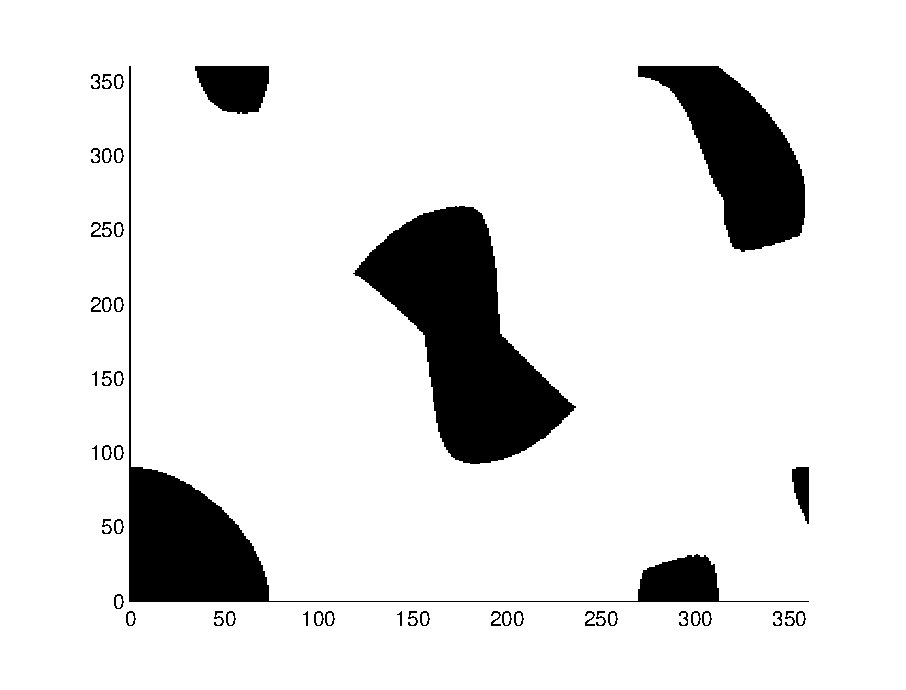
\includegraphics[width=3.5in]{./figures/cspace2.eps}
	\caption{Configuration space \#1, the points presented in table \ref{tbl:pts} were used with this space.}
	\label{fig:space1}
\end{figure}

\begin{figure}[h]
\label{cs2}
	\centering
	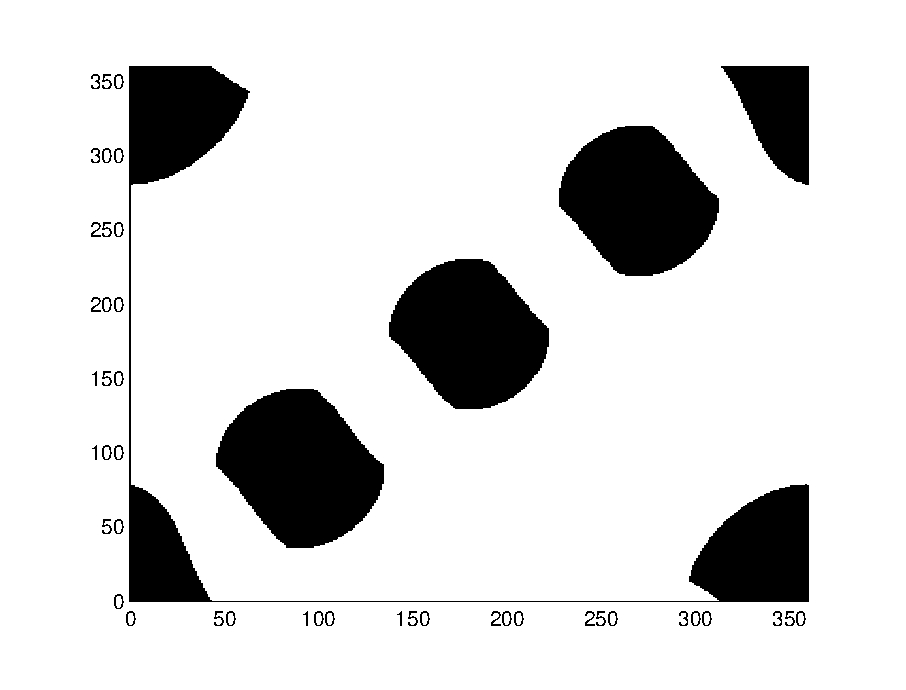
\includegraphics[width=3.5in]{./figures/cspace3.eps}
	\caption{Configuration space \#2, the points presented in table \ref{tbl:pts} were used with this space.}
	\label{fig:space2}
\end{figure}

\begin{figure}[h]
\label{cs3}
	\centering
	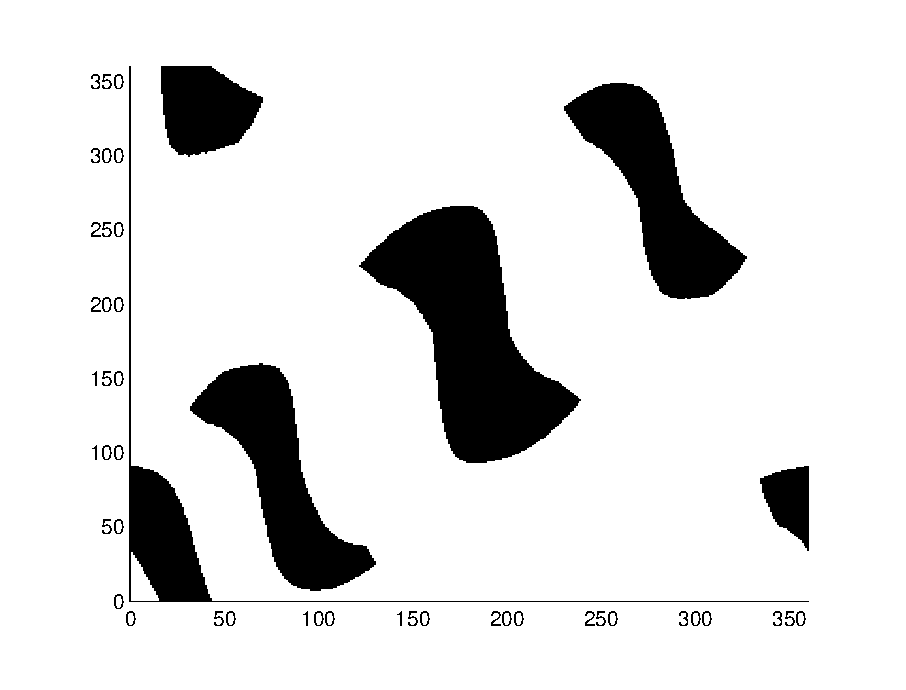
\includegraphics[width=3.5in]{./figures/cspace4.eps}
	\caption{Configuration space \#3, the points presented in table \ref{tbl:pts} were used with this space.}
	\label{fig:space3}
\end{figure}

